\newpage
\section{Sensor}
Sensoren, som blev beskrevet i hardwareafsnittet, skal kommunikere med Arduino boardet. Dette kræver nogle trin som kan findes i databladet til sensoren. På figur \ref{sensor_min} ses et overblik over funktioner lavet i softwaren, som skal til for at aflæse sensoren. Disse funktioner er konstrueret ud fra databladet, hvor det ses at tre trin skal følges præcist for at tilgå sensoren. De tre trin er en initialisering, ROM command og function command. Herefter er sensoren klar til at blive aflæst.



I databladet til DS18B20 sensoren ses et flowchart der viser hvordan mikroprocessoren kommunikerer med sensoren og hvordan den tilgår funktionerne  sensoren kan udføre. Ud fra flowchartet er der konstrueret en mindre version, som indeholder de nødvendige funktioner for at tage en temperaturmåling. Disse funktioner ses på figur \ref{sensor_min}.



\begin{figure}[h!]
  \centering
  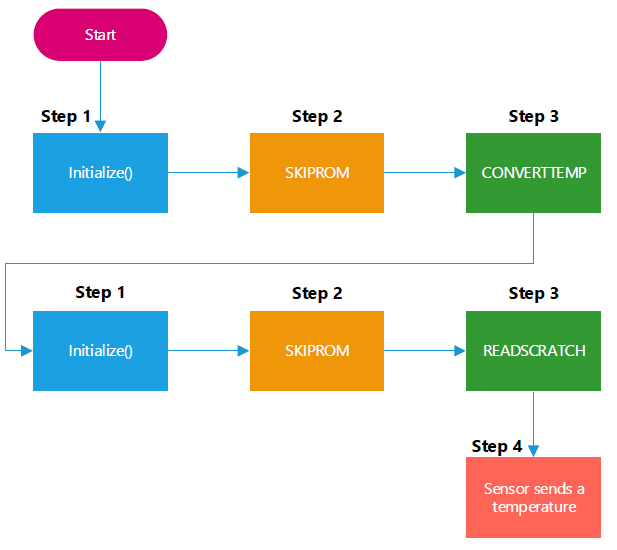
\includegraphics[width=1\textwidth]{figures/sensor_minimum.png}
  \caption{Kommunikation med sensor.}
  \label{sensor_min}
\end{figure}

\newpage
\subsection{initialize()}
Initialiseringsfunktionen, som ses på flowchartet, er konstrueret ved at finde intervallerne som er nødvendige for at tilgå sensoren over en 1-Wire forbindelse. Disse er aflæst af en graf fra databladet (jf. figur \ref{sensor_min}).
\begin{figure}[h!]
  \centering
  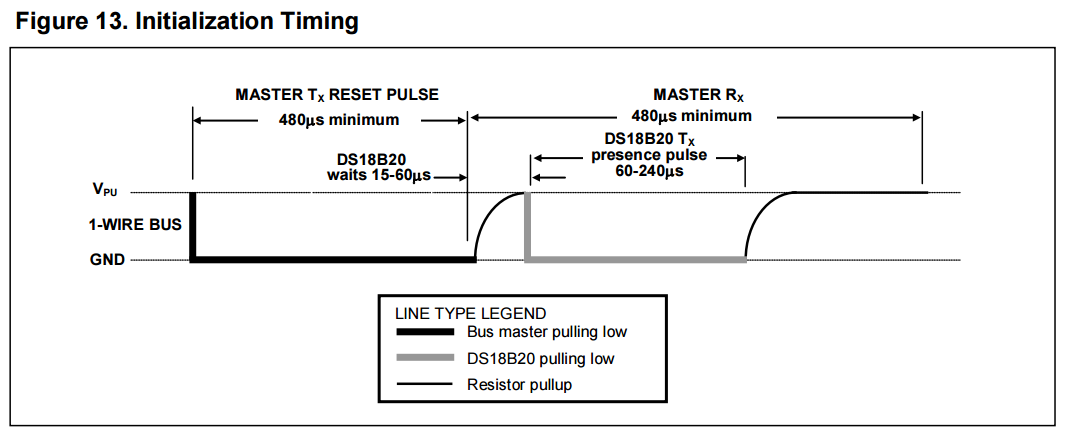
\includegraphics[width=0.9\textwidth]{figures/Initialization_timing.png}
  \caption{Fra datablad om hvordan sensor skal initialiseres.}
  \label{sensor_init}
\end{figure}
\newpage
Fra databladet ses at 1-Wire forbindelsen skal have en reset pulse i minimum 480$\mu$S og en presence pulse vil herefter blive sendt fra sensoren til mikroprocessoren inden for 60-240$\mu$S. Dette gøres ved at sende et low signal som svarer til reset pulsen. Derefter sættes forbindelsen til input, hvor den vil gå i tri-state mode og pull-up modstanden vil trække signalet højt. 
\\
\\
I koden bliver dette gjort ved at kalde digitalWrite() med low som parameter, i kombination med et delay på 500$\mu$S. Derefter sættes pinMode til input og et delay på 500$\mu$S anvendes igen. Dette kan ses på figur \ref{sensor_kode}.

\begin{figure}[h!]
  \centering
  \fbox{\includegraphics[width=1\textwidth]{figures/Init.png}}
  \caption{Initialisering kode.}
  \label{sensor_kode}
\end{figure}

\subsection{writeByte()}
For at sende kommandoer til sensoren er en writeByte() funktion konstrueret. Den er lavet ud fra samme fremgangsmåde som initialize() funktionen ved at aflæse en graf der indeholder de intervaller der skal til for at tilgå sensoren.

\begin{figure}[h!]
  \centering
  \fbox{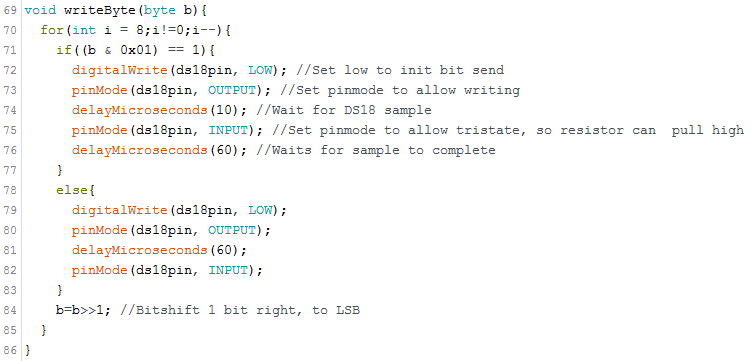
\includegraphics[width=1\textwidth]{figures/write_byte.png}}
  \caption{writeByte() arduino kode.}
  \label{write_byte}
\end{figure}
Det kode som står under if(), er det kode som anvendes hvis der ønskes at skrive et 1 tal og det der står under else(), er det der anvedes til at skrive et 0. Da sensoren modtager 1 bit af gangen, kører for-loopet igennem otte gange . Hver gang en enkelt bit bliver kontrolleret, om der står 1 eller 0, vil der blive foretaget et bitshift til højre og den næste bit vil blive kontrolleret. På denne måde kan der skrives til sensoren.


\subsection{Overblik}

\begin{figure}[h!]
  \centering
  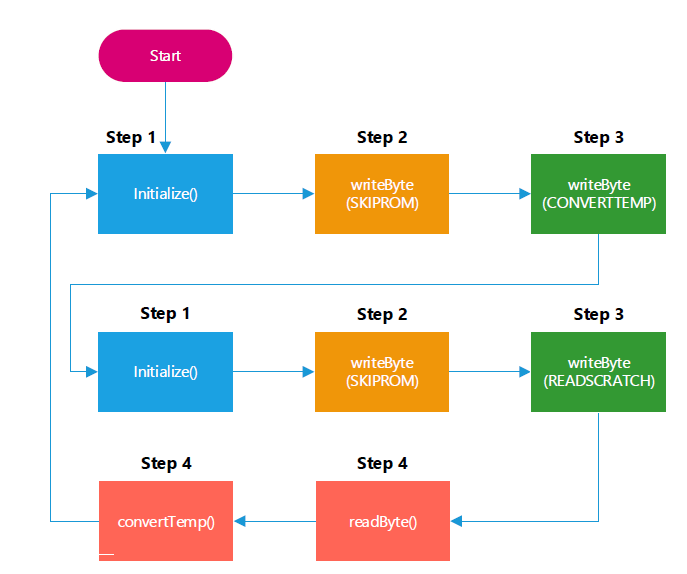
\includegraphics[width=1\textwidth]{figures/sensor_communication.png}
  \caption{De funktioner der skal til for at mikroprocessoren kan kommunikere med sensoren.}
  \label{sensor_total}
\end{figure}